% mnras
% \documentclass[fleqn,useAMS,usenatbib]{mnras}

% apj
%\documentclass[iop, twocolappendix, appendixfloats, numberedappendix, apj]{emulateapj}
\documentclass[iop, twocolappendix, appendixfloats, numberedappendix, apj]{hackemulateapj}
%\documentclass{emulateapj}

%=====================================================================
% CUSTOM: PACKAGES, MACROS & SETTINGS
%=====================================================================
% packages for figures
\usepackage{graphicx,todonotes}

% packages for symbols
\usepackage{latexsym,amssymb}

% AMS-LaTeX package for e.g. subequations
\usepackage{amsmath,morefloats}
\usepackage[backref,breaklinks,colorlinks,citecolor=blue]{hyperref}
\usepackage{natbib,graphicx,amsmath,subfigure,color,xcolor}
%\usepackage{natbib,graphicx,amsmath,subfigure,color,xcolor,hyperref}
\usepackage{verbatim}
\usepackage{threeparttable}

%\usepackage{lineno}
%\linenumbers

\topmargin-1cm

\newcommand\notedo[1]{\todo[color=yellow, inline, size=\small]{To do:#1}}
\newcommand\notewrite[1]{\todo[color=orange, inline, size=\small]{To write: #1}}
\newcommand\noteask[1]{\todo[color=cyan, inline, size=\small]{To ask: #1}}
\newcommand\notecontrib[1]{\todo[color=green, inline, size=\small]{Contributors: #1}}
\newcommand\esstodo[1]{\todo[color=yellow, inline, size=\small]{ESS: #1}}
\newcommand{\ess}[1]{\textcolor{red}{[ESS: \bf #1]}}
\newcommand{\mrb}[1]{\textcolor{purple}{[MRB: \bf #1]}}


\newcommand{\vecg}{\mbox{\boldmath $g$}}
\newcommand{\vece}{\mbox{\boldmath $e$}}
\newcommand{\veck}{\mbox{\boldmath $k$}}
\newcommand{\vecQ}{\mbox{\boldmath $Q$}}
\newcommand{\vecF}{\mbox{\boldmath $F$}}
\newcommand{\vecD}{\mbox{\boldmath $D$}}
\newcommand{\matR}{\mbox{$\bf R$}}
\newcommand{\matC}{\mbox{$\bf C$}}
\newcommand{\bnab}{\boldsymbol{\nabla}}
\newcommand{\bnabg}{\boldsymbol{\nabla_g}}
\newcommand{\galsim}{\texttt{GALSIM}}
\newcommand{\ngmix}{\texttt{ngmix}}
\newcommand{\nnsim}{\texttt{nsim}}
\newcommand{\snr}{$S/N$}
\newcommand{\sn}{$S/N$}
\newcommand{\coadd}{{\rm coadd}}
\newcommand{\desreq}{$4\times 10^{-3}$}
\newcommand{\lsstreq}{$2\times 10^{-3}$}

\newcommand{\mcal}{\textsc{metacalibration}}
\newcommand{\mdet}{\textsc{metadetection}}
\newcommand{\Mcalshort}{\textsc{metacal}}
\newcommand{\Mcal}{\textsc{Metacalibration}}
\newcommand{\Mdet}{\textsc{Metadetection}}
\newcommand{\vest}{\mbox{\boldmath $e$}}
\newcommand{\est}{e}
\newcommand{\mcalR}{\mbox{\boldmath $R$}}
\newcommand{\mcalRS}{\mbox{\boldmath $R_S$}}
\newcommand{\gest}{\mbox{\boldmath $\hat \gamma$}}
\newcommand{\vecgam}{\mbox{\boldmath $\gamma$}}

\newcommand{\sx}{\textsc{Source Extractor}}

\newcommand{\bfd}{\textsc{BFD}}

\newcommand{\vonkarman}{{von K\'arm\'an}~}


%\setuphead[section][before={\testpage[2]}]

%mnras
%\title[\Mdet]{\Mdet: Mitigating Shear-dependent Object Detection Biases with \Mcal}

%\author[Sheldon et~al.]{Erin Sheldon$^1$, Matthew R. Becker$^2$,
%Niall MacCrann$^{3,4}$, Michael Jarvis$^5$
%  \\$^1$Brookhaven National Laboratory, Bldg. 510, Upton, NY 11973, USA
%  \\$^2$High Energy Physics Division, Argonne National Laboratory, Lemont, IL 60439, USA
%  \\$^3$Center for Cosmology and Astro-Particle Physics, The Ohio State University, Columbus, OH 43210, USA
%  \\$^4$Department of Physics, The Ohio State University, Columbus, OH 43210, USA
%  \\$^5$Department of Physics and Astronomy, University of Pennsylvania, Philadelphia, PA 19104, USA
%}


% apj
\shorttitle{Metacalibration in LSST}
\shortauthors{Sheldon, Becker, Armstrong}

\begin{document}
% mnrad
% \date{Draft \today}

% mnras
%\maketitle

% apj
%\title{\Mdet: Mitigating Shear-dependent Object Detection Biases with \Mcal}
\title{Metacalibration in LSST}

\author{Erin S. Sheldon}
\affil{Brookhaven National Laboratory, Bldg 510, Upton, New York 11973, USA}
\author{Matthew R. Becker}
\affil{High Energy Physics Division, Argonne National Laboratory, Lemont, IL 60439, USA}
\author{Robert Armstrong}
\affil{Lawrence Livermore National Laboratory, Livermore, CA 94551, USA}


\begin{abstract}

    \Mcal\ for LSST

\end{abstract}

\section{Introduction}

blah

\section{Results}


% 
\begin{table}
\centering
\begin{threeparttable}
      \caption{
      nostack: the LSST DM stack was not used; d: dithers; r: rotations; c: cosmic rays;
      b: bad columns; R: realistic galaxy properties and noise; v: variable pixel scale
      and WCS shear; p: psf $g_2 = 0.02$; RIZ: $r, i$ and $z$ bands used; LD: large dithers;
      VP: spatially variable moffat PSF.
      }
 \label{tab:shearmeas}

  \begin{tabular}{lcc}
    \hline
    \noalign{\vskip 1mm}
    Simulation & m (99.7\% conf.) & c (99.7\% conf.) \\
     &  $[10^{-3}]$ & $[10^{-5}]$ \\
    \noalign{\vskip 1mm}
    \hline
    \noalign{\vskip 1mm}
        nostack & -0.2 $< m_1 <$ 1.1 & -\\
        d & -1.0 $< m_1 <$ 0.6 & -\\
        dr & -0.6 $< m_1 <$ 1.0 & -\\
        drc & -0.2 $< m_1 <$ 1.2 & -\\
        drcb & -0.9 $< m_1 <$ 0.6 & -\\
        drcbR & -0.9 $< m_1 <$ 0.7 & -\\
        drcbv & -0.9 $< m_1 <$ 0.7 & -\\
        drcbvp & -0.9 $< m_1 <$ 0.7 & $-1.8 < c_2 < 1.2$\\
        drcbvpRIZ & -0.5 $< m_1 <$ 0.6 & $-1.5 < c_2 < 1.4$\\
        drcbvpLD & -0.8 $< m_1 <$ 0.9 & $-1.7 < c_2 < 1.5$\\
        drcbvRIZVP & -0.6 $< m_1 <$ 1.0 & $-1.8 < c_2 < 1.3$\\

    \noalign{\vskip 1mm}
    \hline
  \end{tabular}

    \end{threeparttable}
\end{table}



\begin{figure}
    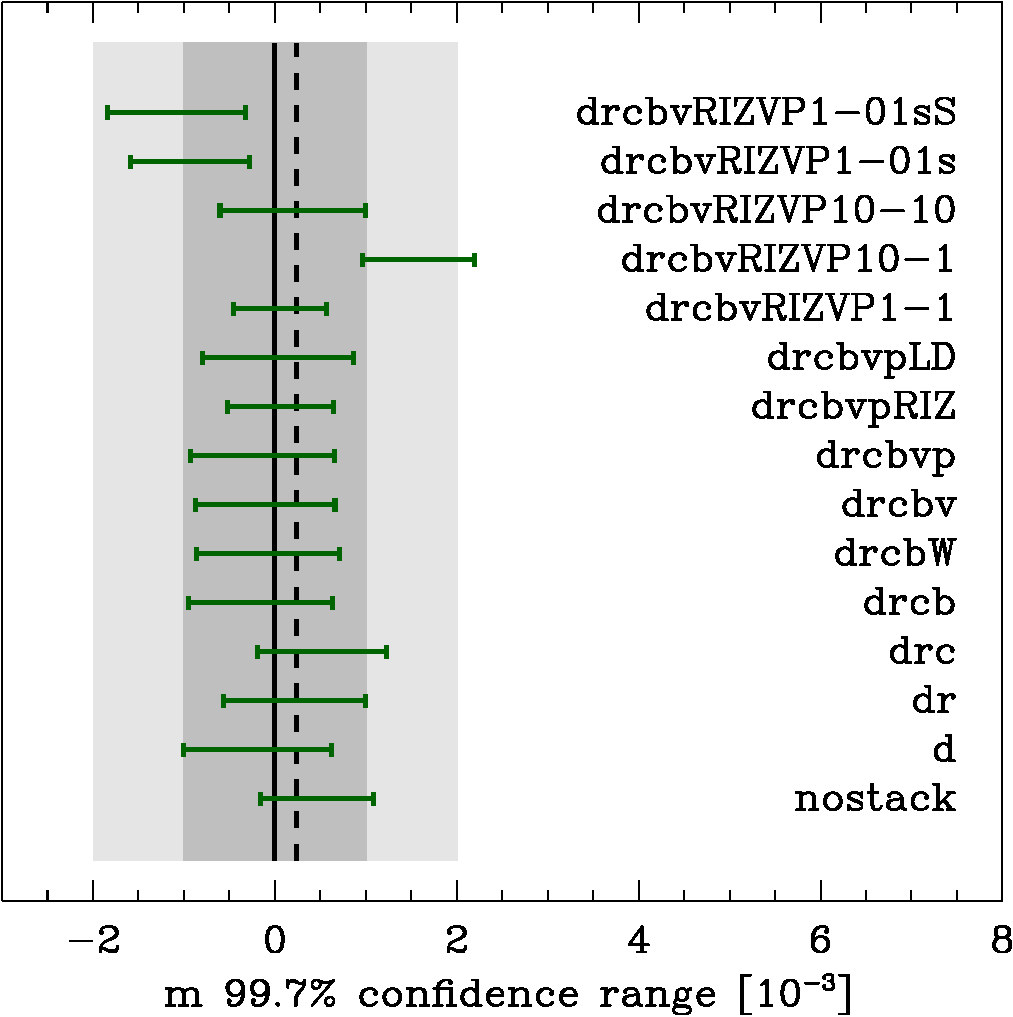
\includegraphics[width=\columnwidth]{code/mvals.pdf}
    \caption{99.7\% confidence range for the multiplicative bias $m$ in
     various simulations.  The light gray region represents the total
     error budget for LSST, the dark gray region represents our target.
     The dashed line is the expected bias due to second order shear effects.  Each
     point represents the $m$ value measured in a particular simulation.  To the right
     of each point is a code representing the simulation features used, which are
     nostack: the LSST DM stack was not used; d: dithers; r: rotations; c: cosmic rays;
     b: bad columns; W: realistic galaxy properties and noise using
      the WeakLensingDeblending package; v: variable pixel scale
     and WCS shear; p: psf $g_2 = 0.02$; RIZ: $r, i$ and $z$ bands used; LD: large dithers;
     VPX-Y: spatially variable moffat PSF with X times the expected variation for LSST,
     and Y epochs per band;  s: stars included, S: star masks and bleeds
     included.
    }
\end{figure}

\begin{figure}
    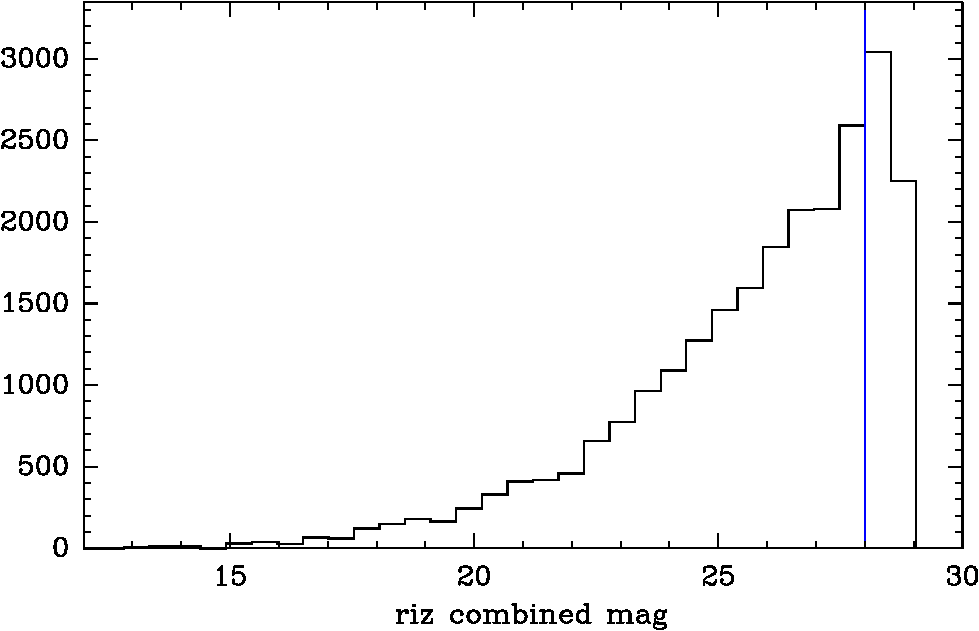
\includegraphics[width=\columnwidth]{mag-hist.pdf}
    \caption{
        Star magnitudes measured in simulated $r+i+z$ combined coadds.  The
        $r-band$ magnitude limit for the input star sample is shown as a
        vertical line at 28.  The detection in the combined image is
        somewhat deeper.
    }
\end{figure}



\section*{Acknowledgments}

ES is supported by DOE grant DE-AC02-98CH10886, and MB is supported by DOE
grant DE-AC02-06CH11357.  RM is supported by the US Department of Energy Cosmic
Frontier program, grant DE-SC0010118.


%\bibliographystyle{mnras}
%\bibliography{references}
%\bibliography{apj-jour,references}
%\bibliographystyle{apj}
\bibliographystyle{aasjournal}
\bibliography{references}

\end{document}
